\label{sec:methods}
\section{Methods and Materials}

GOPR was designed incrementally, slowly testing each improvement to the design at each step, to ensure the inner workings of the reactor were understood and minimizing errors in optimization.  Initially, core behavior and criticality in response to enrichment, core alloy material, and size where determined. After that, moderating materials and the interaction with the shell was tested and a rough design was decided upon, that was to be optimized. As a benchmark, a more conventional version was created that retained some of the concepts GOFR was intended to leverage for greater flux. In both, success was measured by a critical core and a FMESH tally located in the beam port of the reactor. A general geometry for GOFR was developed and coded into MCNP after signifigant geometric calculations and was changed only slightly after testing.

\subsection{Core and Moderator}

After considering several variations of reactors, initally GenIV power reactors and then various research sources, it was decided to use standard low enriched uranium (LEU), due to its characteristics of being well studied and relatively simple to refine and use. As a benchmark, 80\% enriched uranium was used, chosen to be under the weaponization threshold of 90\% but still highly enriched. This allowed for the comparision of designs by giving a clear goal for criticality and flux. Furthermore, LEU fuel of 20\% enrichment, and two half uranium and half alloy core compositions were tested. Initially, naked cores were tested to see the exact influence of size on the criticality and to further compare the improvements made by any additions. First was the moderating material, the material that encased the core and filled out the space between the core and the reflecting shell. It was not yet certain if the geometric approach would work, so a variety of moderators were examined. As seen in table \ref{tab:pure}, water was very good at reducing the energy of the neutrons enough to raise the criticality but would be a hinderance to the geometric approach as it relied on neutrons traveling largely undisturbed. For that purpose, aluminum performed well, only slightly altering the criticality. Vacuum, as seen in table \ref{tab:purevac}, performed the best in unaltering criticality as it showed no interaction with neutrons, which was a result used as another benchmark. These results are consistent with the data from NIST on neutron scattering lengths and were already largely factored into design considerations. These simulations are to confirm that the models and effects used in the design of GOFR were well founded in reality, using MCNP as a surrogate for reality.

As a result of these simulations, it was decided that GOFR would use aluminum as the moderating filling and the conventional-style reactor would use water. The use of water in this case is consistent with the majority of research oriented reactors. Next was the shell material. A brief and oversimplified test of possible materials was done, in which a sphere of the reflector material was placed around the core and the criticality was compared. A thickness was arbitrarily chosen such that signifigant neutrons would not escape. Graphite was then chosen for further development, rather than beryillium, zirconium hydride, water, or heavy water for both criticality and geometric design considerations.

A rough volume to enrichment relationship, shown in table \ref{tab:variations}, was used to decide how enriched the uranium would be and still be critical. It was decided to adhere to the general standard of having sub-20\% enrichment to maximize flux while maintaining safety but did not go as low as some reactors do. Using this minimum volume of LEU, alloys and geometries could be explored without too much iteration in running MCNP code. For the conventional style reactor, a cube, side length of $1=30cm$, was used and its enrichment, 15\%, was determined by this value. For GOFR, a sphere made of 50\% uranium at just below the 20\% limit, 19.9\%, the radius had to be $r=25cm$ to achieve criticality upon introduction of the shell.\footnote{For a full listing of tables and results, see section \ref{sec:results}}

\subsection{Shell}

The surrounding shell and its geometry has three purposes:

\begin{enumerate}
	\item Increasing criticality.
	The generated neutrons that manage to escape the core do not need to be wasted. By sending more back into the core, the reactor can fission more than would be expected as if it was a larger, more intrinstically critical piece of uranium.
	\item Neutron reflection.
	The neutrons that are generated do not need to continue radiating isotropically. By biasing how neutrons travel in the reactor, more of the generated neutrons can pass through the beam port, giving off a flux much higher than a similarly powerful reactor.
	\item Thermal regulation.
	Any heat generated by the fission reactions in the core is transported out to the shell where it can be more easily regulated. The exact workings and optimizations for this are outside the scope of the project but some discussion is given in section \ref{sec:future}.
\end{enumerate}

\subsubsection{Increasing Criticality}

Any material upon which neutrons scatter can be used for moderation and reflection to this end. The only requirements are that the core be surrounded and that there is no path out of the reactor, especially if scattering is elastic. As long as more neutrons hit the core that otherwise would not have, the criticality will increase, and even more neutrons will be produced.

\subsubsection{Neutron reflection}

Neutrons do not behave like light and reflecting them is not as simple. However, with certain materials and angle, reflection is largely elastic and therefore reflected neutrons follow a general trajectory with a higher incidence along the central path. Therefore, neutrons will differ from light in terms of path mostly in a rather tight distribution around this central path. This general logic was used when designing GOFR.
Initally, a parabolic reflector was considered as it is a common optical tool. It would take a radiant source located at the focal point and direct its now collimated beam foward. That would be perfect, if the reactor was small and the irradiation window was much larger, because it turns an isotropic source into a linear one and collimates the beam, as seen in figure \ref{fig:parabola}. Unfortunately, this would not fit the application. 

\begin{figure}[!htbp]
\caption{Parabolic reflector}
\label{fig:parabola}
\centering
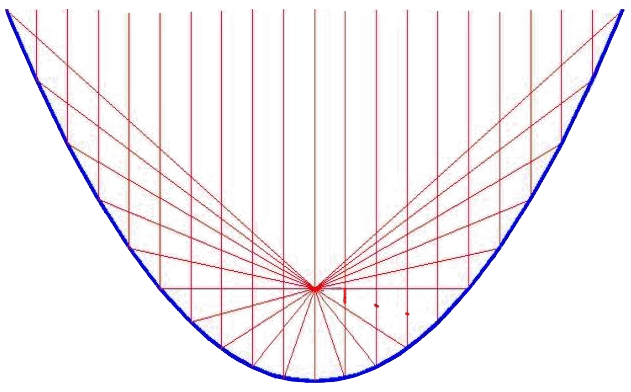
\includegraphics[width=0.75\textwidth]{parabola.png}
\end{figure}

Next a sphere was considered, as its surface is perfectly perpendicular at every radial line and that is exactly the use case with increasing criticality. However, this does nothing to promote a mass exodus of neutrons and creating a high flux beam. This is where the development of the conventional reactor essentially ended. In the conventional reactor, the core was placed against one side of the shell and the beam port where the core met the shell. This allowed for most of the generated neutrons to support continuing fission while a signifigant amount were shuttled out of the reactor, as seen in figure \ref{fig:structure}.

\begin{figure}[!htbp]
\caption{Core and shell structures of Conventional Reactor}
\label{fig:structure}
\centering
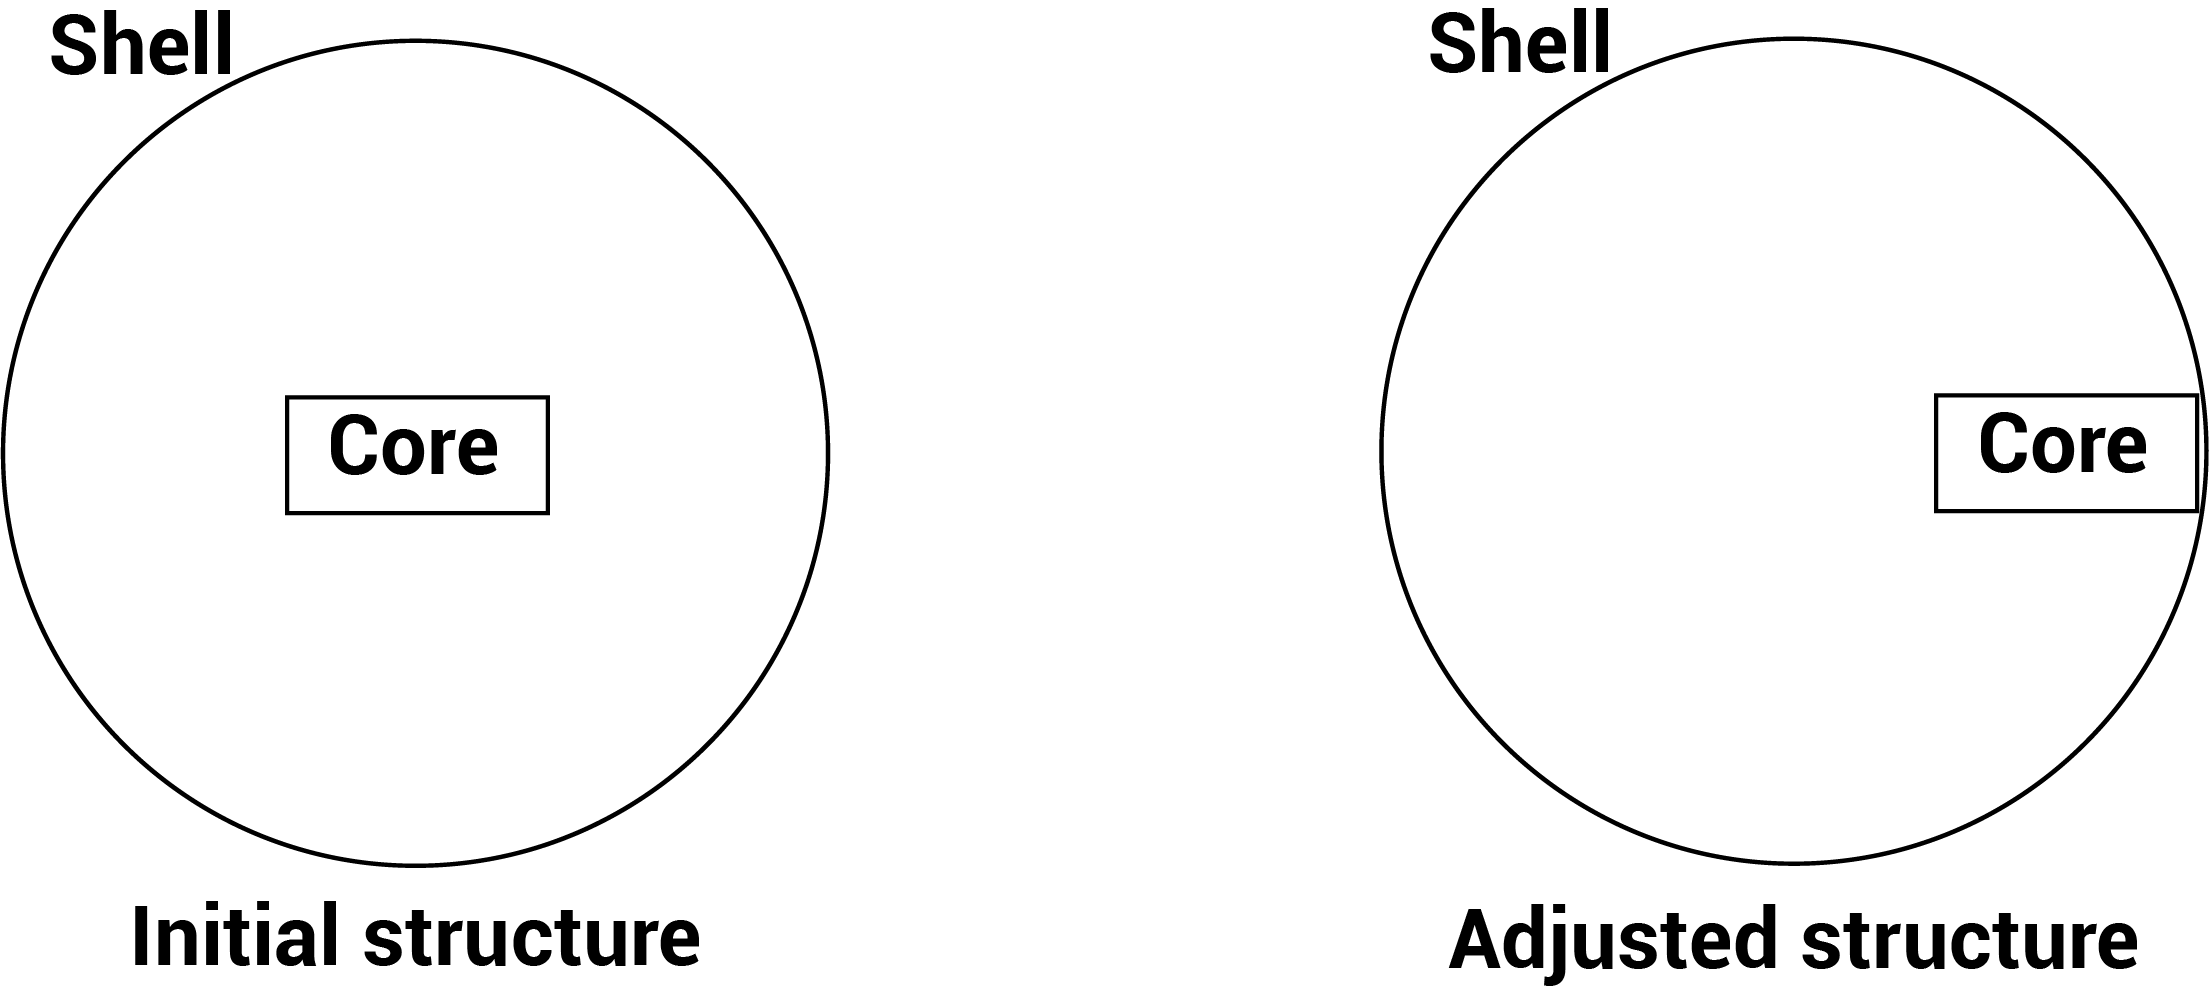
\includegraphics[width=0.75\textwidth]{structure.png}
\end{figure}

For GOFR, it seemed that the answer was in the geometry of the reflector. To that end, an ellipsoidal reflector was developed, the size and shape based upon data from the tests on the core composition. An ellipsoid has two focal points, and anything radiating isotropically from one, irraditates the other perfectly uniformly, as seen in figure \ref{fig:ellipsoid}.

\begin{figure}[!htbp]
\caption{Ellipsoidal reflector}
\label{fig:ellipsoid}
\centering
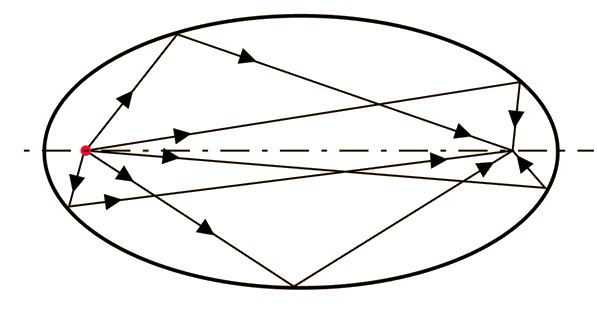
\includegraphics[width=0.75\textwidth]{ellipsoidal.png}
\end{figure}

Since the aim was to maximize neutrons leaving the reactor, an ellipsoidal shell was not the entire solution. To accomplish that, a conical reflector was fitted to the midpoint of the ellipsoid, its surface angle matching the path of any neutrons that reflect off of the ellipsoidal reflector at the junction of the two surfaces. This ensured that the focal point of the neutron radiation was inside the beam port, ensuring that the majority of the generated neutrons would escape the reactor. The conical reflector further ensured that enough neutrons would return to the core by acting as a conventional reflector. This geometric concept is illustrated in figure \ref{fig:design02}.

\begin{figure}[!htbp]
\caption{GOFR concept design}
\label{fig:design02}
\centering
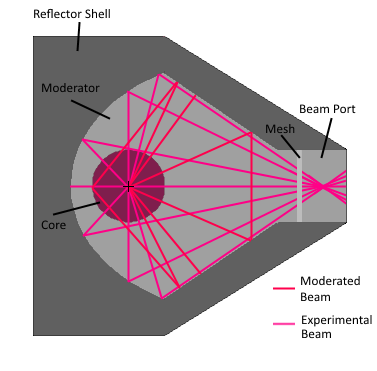
\includegraphics[width=0.75\textwidth]{design-02.png}
\end{figure}

\subsubsection{Particle interaction}

Thermal regulation is outside the scope of this project but aluminum conducts heat very well and would conduct heat away from the core and deposit it in the shell, where coolant can be pumped on or through the shell. This allows the core to function at higher wattage without damage and thus create higher neutron flux. By running water over the shell's surface and through cavities or pipes inside the shell, heat can be extracted efficently. More discussion is given in section \ref{sec:future}.

\subsection{Beam Port and Tally}

In both designs, the neutrons were directed towards the beam port, a hole in the shell in which a collimator can be inserted. The raw beam was recorded and analyzed by means of a FMESH tally, which counted the neutrons passing through the beam port and their direction. From this, the beam behavior and raw flux can be calculated. This can then be compared to existing sources and the feasibility of this design can be ascertained and gauged.
